
%%%%%%%%%%%%%%%%%%%%%%% file typeinst.tex %%%%%%%%%%%%%%%%%%%%%%%%%
%
% This is the LaTeX source for the instructions to authors using
% the LaTeX document class 'llncs.cls' for contributions to
% the Lecture Notes in Computer Sciences series.
% http://www.springer.com/lncs       Springer Heidelberg 2006/05/04
%
% It may be used as a template for your own input - copy it
% to a new file with a new name and use it as the basis
% for your article.
%
% NB: the document class 'llncs' has its own and detailed documentation, see
% ftp://ftp.springer.de/data/pubftp/pub/tex/latex/llncs/latex2e/llncsdoc.pdf
%
%%%%%%%%%%%%%%%%%%%%%%%%%%%%%%%%%%%%%%%%%%%%%%%%%%%%%%%%%%%%%%%%%%%


\documentclass[runningheads,a4paper]{llncs}

\usepackage{amssymb}
\setcounter{tocdepth}{3}
\usepackage{graphicx}
\usepackage[affil-it]{authblk}
\usepackage[utf8]{inputenc}
\usepackage{cite}
%\usepackage[numbers]{natbib}
\usepackage[english, main=ngerman]{babel}% deutsche Trennregeln
%\usepackage[T1]{fontenc}% wichtig für Trennung von Wörtern mit Umlauten
\usepackage{microtype}% verbesserter Randausgleich
\usepackage[hidelinks]{hyperref}
\usepackage{multirow}
\usepackage{float}

\usepackage{graphicx}
\graphicspath{ {./img/} }

\usepackage{url}
%\urldef{\mailsa}\path|{alfred.hofmann, ursula.barth, ingrid.haas, frank.holzwarth,|
%\urldef{\mailsb}\path|anna.kramer, leonie.kunz, christine.reiss, nicole.sator,|
%\urldef{\mailsc}\path|erika.siebert-cole, peter.strasser, lncs}@springer.com|    
\newcommand{\keywords}[1]{\par\addvspace\baselineskip
\noindent\keywordname\enspace\ignorespaces#1}
\renewcommand{\labelitemi}{$\bullet$}
\renewcommand{\labelitemii}{$\cdot$}
\renewcommand{\labelitemiii}{$\diamond$}
\renewcommand{\labelitemiv}{$\ast$}

\begin{document}

\mainmatter  % start of an individual contribution

% first the title is needed

\title{Virtuelles Museum\\Analyse\\ Prototyping\\ Evaluation}

% a short form should be given in case it is too long for the running head
\titlerunning{Virtuelles Museum}

% the name(s) of the author(s) follow(s) next
%
% NB: Chinese authors should write their first names(s) in front of
% their surnames. This ensures that the names appear correctly in
% the running heads and the author index.
%

\author{
		Adrian Franken (Matr.nr.:s0538115),\\
		Chris-Andr\'{e} Posselt (Matr.nr.:s),\\
		Elsa Buchholz (Matr.nr.:s0544180),\\ 
		Igor Olegovich Turanin (Matr.nr.:s0549350)
	   }

%
\authorrunning{Virtuelles Museum}
% (feature abused for this document to repeat the title also on left hand pages)

% the affiliations are given next; don't give your e-mail address
% unless you accept that it will be published
%\institute{Hochschule für Technik und Wirtschaft Berlin\\}
\institute{
		Hoschschule für Technik und Wirtschaft Berlin\\
}
\affil{	
		Fachbereich: Informatik, Kommunikation und Wirtschaft\\
		Studiengang: Angewandte Informatik\\
		Seminar: Human-Computer Interaction\\
		Seminarverantwortlicher: Prof. Dr.-Ing. Johann Habakuk Israel \\
}


%
% NB: a more complex sample for affiliations and the mapping to the
% corresponding authors can be found in the file "llncs.dem"
% (search for the string "\mainmatter" where a contribution starts).
% "llncs.dem" accompanies the document class "llncs.cls".
%

%\toctitle{Lecture Notes in Computer Science}
%\tocauthor{Authors' Instructions}

{\def\addcontentsline#1#2#3{}\maketitle}
\renewcommand{\contentsname}{Inhaltsverzeichnis}
%\maketitle
%\thispagestyle{empty}
\newpage
%\thispagestyle{empty}
\tableofcontents
\newpage
\thispagestyle{empty}
\listoffigures
\newpage
\thispagestyle{empty}
\listoftables
\newpage
\setcounter{page}{1}

\selectlanguage{english}
\begin{abstract}
	

\keywords{}
\end{abstract}
\selectlanguage{ngerman}

\section{Einleitung}
\section{Anforderungsanalyse}
\subsection{Anwendungsfälle und Nutzungskontext} \label{sect:anwendung}
Laut Miedler 2010 ist ein Museum eine Einrichtung, die zu Bildungs- und Forschungszwecken Zeugnisse von Umwelt und Menschen, der Öffentlichkeit zur Verfügung stellt und aufbewahrt. Die Zeugnisse von Umwelt und Menschen können sehr vielfältig sein. Dabei kann es sich um Bauarten wie Schlösser und Burgen handeln, als auch um Kunstobjekte aus der Malerei oder Fotografie sowie naturwissenschaftliche oder technische Erzeugnisse. Somit lassen sich Museen in verschiedene Arten einteilen, wie beispielsweise in Burg- und Schlossmuseum, Kunstmuseum, technisches oder naturkundliches Museum. Nicht nur der Bildungs- und Forschungszweck eines Museums soll erfüllt werden, sondern das Erleben der Zeugnisse soll innerhalb einer Ausstellung erreicht werden. Ausstellungen können dabei dauerhaft oder wechselnd kuratiert werden, wobei sie je nach Art des Museums an einem bestimmten Ort gebunden sind. Aufgrund der Vielzahl von Museumsarten und dem Zweck des Bildungs- und Forschungsauftrages bzw. Erlebnisses, besitzen Museen eine weitgefasste Zielgruppe. Daraus ergeben sich Interessengruppen, die sich aus der jeweiligen Art des Museums oder aus verschiedenen Berufsgruppen wie beispielsweise Lehrer, Schüler, Studenten oder Mitarbeiter des Museums wie Kuratoren oder Archivare  ergeben\cite[S. 29]{Miedler.2010}.\\ 

In der folgenden Tabelle werden die Stakeholder des Systems zusammengefasst. Sie beschreibt welches Interesse und welchen Einfluss die Stakeholder auf das System haben.\\

\begin{table}
	\begin{tabular}{|c|c|c|}\hline
	Stakeholder & Interesse & Einfluss\\ \hline
	\multirow{2}*{aktive Museumsgänger} & neue Möglichkeiten &\\  & zur Erkundung der Exponate ermöglichen & sehr hoch \\ \hline
	
	nicht aktive Museumsgänger & Interesse am Museumsbesuch wecken  & hoch\\ \hline
	
	\multirow{2}*{Archivar des Museums}& Erfassung der Exponate &\\ & innerhalb einer Datenbank & sehr gering\\ \hline
	
	\multirow{2}*{Kurator des Museums} & Integration von Technologien&\\& innerhalb einer Ausstellung & hoch\\ \hline
	pädagogische Kräfte  & Lehreiche Informationen erhalten& sehr hoch\\ \hline
	Kinder  & spielerischer Umgang mit den Exponaten & sehr hoch\\ \hline
	\end{tabular}
\end{table}

Daraus ergeben sich folgende Ziele:
\begin{itemize}
	\item Aktive Museumsgänger sollen weiterhin motiviert werden in das Museum zu gehen und durch neue Technologien mit den Exponaten interagieren können. Die Interaktion soll dem Kenner des Museums ermöglichen, neue Informationen bzw. einen neuen Zugang zu diesen zu gewinnen.
	\item Nicht aktive Museumsgänger sollen durch neue Technologien einen Zugang zum Museum erhalten, wobei das Interesse für die Exponate geweckt werden soll.
	\item Mitarbeiter des Museums sollen von den Technologien profitieren, indem sie Exponate besser Verwalten können bzw. die Ausstellung mit einem höheren Gehalt an Interaktionen konzipieren können.
	\item Pädagogische Kräfte sollen Wissen mit Hilfe des Museums verständlicher vermitteln können.
	\item Kinder sollen spielerisch Lernen können und mit Freude das Museum als Lernraum entdecken.\\
	
\end{itemize}

Das virtuelle Museum kann die Grenzen des Ortsbezuges aufheben. Beispielsweise kann ein virtuelles Museum über das Internet erreichbar sein, sodass die Ausstellungsstücke unabhängig von einem bestimmten Ort zugänglich sind. Aufgrund des Standes der Technik ist es möglich das Erleben der Ausstellungstücke durch das Interagieren und Herstellen von Zusammenhängen im virtuellen Raum greifbar zu machen. Durch das Bereitstellen von Informationen im virtuellen Raum auf individuelle Art und Weise kann vor allem dem Bildungsanspruch entsprochen werden und somit im besonderen der Zielgruppe Lehrer und Schüler entsprochen werden. Mitarbeiter eines Museums wie beispielsweise Kuratoren oder Archivare könnten vom virtuellen Museum profitieren innerhalb einer dreidimensionalen Datenbank als Überblick zur Verwaltung und zum Austausch von Ausstellungsstücken oder beim virtuellen zusammenstellen von Ausstellungen. Im folgenden Abschnitt zeigt der Stand der Technik weiterführende Möglichkeiten wie ein virtuelles Museum verstanden werden kann.\\

\subsection{Stand der Technik} \label{sect:standtechnik}

Eine Kategorie wie ein virtuelles Museum verstanden werden kann, ist das Online-Museum. Darunter können Museen fallen, die im Internet virtuell, begehbar und interaktiv nutzbar sind. Ein Beispiel dafür ist das Google Art Projekt \cite{GoogleCultureInstitut.2011}. Es ermöglicht Ausstellungshäuser weltweit zu erkunden. Auf dieser Seite können sich Nutzer durch die Bestände der Museen klicken und eigene Galerien anlegen, sowie virtuelle Rundgänge durch die Museen machen. Ziel eines Online-Museums ist es die Nutzer in das entsprechende Museum zu locken.\\ 

Die zweite mögliche Kategorie virtuelle Museen einzuordnen ist das VR-Museum. Dabei wird die VR-Technologie verwendet, um Nutzer mittels einer App und einer VR-Brille einen Museumsbesuch zu ermöglichen. Diese Variante ist Ort- und Zeitunabhängig. Das Museum für Naturkunde in Berlin verwendet die Technologie, um einen Dinosaurier zum Leben zu erwecken. Dabei kann der Besucher sich vor Ort eine VR-Brille ausleihen oder via App Ortsunabhängig sich den Dinosaurier ansehen. In einer dritten Kategorie können mittels AR-Technologie sich auf einem Tablet zusätzliche Informationen zu Ausstellungsstücken angezeigt werden, sowie es das Bayerische Nationalmuseum in München macht \cite{GoetheInstitute.V..2017}.\\

Im Bereich der 3D-Druck Technologie können Ausstellungsstücke als 3D-Objekt ausgedruckt werden. Das Projekt Museum in a Box verleiht gedruckte 3D-Objekte aus einem Museum in einer kleinen Box. Die Ausstellungsstücke in Miniformat kommunizieren über das Internet, um Informationen zu einem bestimmten Objekt abzurufen und sprachlich wiederzugeben. Somit werden die Ausstellungsstücke anfassbar und können in einen bestimmten Kontext gestellt werden \cite{GeorgeOates.2015}.\\

Im Bereich der Tangible Interfaces Technologie kann die 3D-Druck Technologie verwendet werden, um 3D-Ausdrucke von Ausstellungsstücken als Interface zu nutzen. Die 3D-Objekte sind mit Sensoren und Elektronik ausgestattet, sodass mit Ausstellungsstücken interagiert werden kann \cite{Capurro.2015}.\\ 

Zusammenfassend lässt sich sagen, dass die Technologien 3D-Druck, Augmented Reality (AR) und Virtuell Reality (VR) es ermöglichen ein virtuelles Museum auf unterschiedlichste Art und Weise entstehen zu lassen. Dabei können die Technologien ein Museum virtuell ergänzen oder es gänzlich ersetzen. Die Interaktion innerhalb eines virtuellen Museums ist mit Tangible User Interfaces denkbar, bei dem dreidimensionale Objekte mit Hilfe von einem anfassbaren Objekt die virtuellen Ausstellungsstücke bewegt und gesteuert werden. Der 3D-Druck kann Ausstellungsstücke in Miniformat haptisch erlebbar und zu einem Sammelobjekt, das mit einem Informationsgewinn verknüpft wird, gemacht werden. Die Technologie AR kann ein Museum ergänzen, indem Ausstellungstücke in einen virtuellen Kontext gesetzt werden oder mit Informationen versehen werden, die der Nutzer sich individuell anpassen kann. Der Nutzer kann entscheiden, wie die Information ausgeben wird. Vorstellbar ist, dass die Sprache oder Textform, die Tiefe der Information und die Geschwindigkeit der Darstellung gewählt werden können. Im folgenden Abschnitt werden die Ziele und Ergebnisse der durchgeführten Fokusgruppe zum Thema virtuelle Museen vorgestellt.\\

\subsection{Fokusgruppe}
Im Rahmen der Fokusgruppe wurde untersucht, wie die Interaktion mit den Ausstellungsstücken in einem virtuellen Museum gestaltet werden kann. Dafür wurde zunächst erörtert wie ein klassischer Museumsbesuch und die Interaktion mit den Ausstellungsstücken aussieht. Im zweiten Schritt wurde herausgearbeitet wie in einem virtuellen Museum die Interaktion mit den Ausstellungsstücken aussehen könnte. Ziel war es herauszufinden wie sich die Nutzer ein interaktives Museum vorstellen, welche Technologien dafür verwendet werden sollten und wie die Interaktion mit Hilfe entsprechender Technologien auf ein virtuelles Museum anwendbar ist.\\

Insgesamt waren vier Teilnehmer an der Fokusgruppe beteiligt. Jeder der Teilnehmer war schon einmal in einem Museum, wobei drei der Teilnehmer mindestens zweimal im Jahr ins Museum gehen. Dabei handelt es sich vor allem um Kunstmuseen oder Fotoausstellungen.\\

Die Fokusgruppe wurde von einem Komoderator und einem Moderator geführt und von zwei Protokollanten schriftlich festgehalten. Nach einer inhaltlichen Einleitung haben sich die Teilnehmer vorgestellt, indem sie die Fragen beantworten sollten was der Anlass eines Museumsbesuch ist und welche Erfahrungen sie bisher während eines Museumsbesuchs gemacht haben. Nach der Vorstellungsrunde wurden zur Weiterentwicklung des Gesprächs folgende offene Fragen beantwortet, die sich an einem halboffen Leitfaden orientierten:
\begin{itemize}
	\item Was erwarte ich von einem guten Museumsbesuch?
	\item Wie sollen die Ausstellungsstücke präsentiert werden?
	\item Wie sieht ein Museumsbesuch aus? Gibt es Vor- oder Nachbereitungen?
	\item Wie agiert ihr mit den Ausstellungsstücken?
\end{itemize}

Als gute Museen wurden das Mathematikum Gießen, das Naturkundemuseum Berlin und das jüdische Museum Berlin benannt. Das Mathematikum begeistert, da in Form von interaktiven Experimenten Mathematik erlebt werden kann, wohingegen das Naturkundemuseum vor allem durch seine Ausstellungsstücke wie den Dinosaurier in Lebensgröße besticht. Beeindruckend ist das Jüdische Museum, weil es mit begehbaren Installationen die Ausstellungsstücke erlebbar macht.\\

Grundsätzlich wird ein Museum auf Reisen bzw. im Urlaub besucht ohne Vor- oder Nachbereitungen, sondern eher spontan. Dabei wird Kunst als interessant bezeichnet und am ehesten werden Fotoausstellungen besucht. Innerhalb des Museums wird sich treiben gelassen und durch die Ausstellungsräume geschlendert. Dabei werden die Tafeln für den Informationsgewinn gelesen. Ein Museumsbesuch sollte Lehrreich sein, wobei Interaktionen nicht wichtig sind. Weiterhin wird das Museum gerne genutzt, um  Freunde zu treffen und gemeinsam über die Ausstellungsstücke zu sprechen. Wenn es was zum Anfassen gibt, wird das gerne ausprobiert. Meist wird mit den Ausstellungsstücken durch Beobachtungen interagiert.\\

Nach der Diskussion wurde das Video Museum in a Box gezeigt, indem die Organisation ihr Konzept vom Museum in der Box darstellt. Das Video dient als Überleitung zu virtuellen Museen als eine neue Form der Museen mit veränderten Möglichkeiten zur Interaktion mit Ausstellungsstücken. Im folgenden wurde der Frage nachgegangen wie sie sich ein virtuelles Museum vorstellen und wie darin mit Ausstellungsstücken interagiert werden kann.\\

In Form einer Diskussion haben die Teilnehmer die Kategorien eines virtuellen Museum aus dem Abschnitt \nameref{sect:standtechnik} herausgearbeitet und bewertet. Die Tabelle fasst die Ergebnisse dieser Diskussion zusammen.\\

\begin{table}
\begin{tabular}{|c|c|}\hline
	\textbf{Kategorie}							& \textbf{Beurteilung}\\ 
										\hline
	\multirow{2}*{Online-Museum}		& negativ bewertet,\\
						  				& da viel verloren geht aus dem Museum \\  \hline 
	\multirow{5}*{Virtual Reality}		& innerhalb eines Museums negativ, weil man\\
	                                    & das zu Haus machen kann\\
	                      				& Technik selber als positiv bewertet, weil\\
	                      				& damit unmögliches möglich gemacht werden kann\\
	                     				& unerreichbare Orte sind damit erreichbar\\ \hline
	\multirow{3}*{Augmented Reality}	& positiv in einem Museum,\\ 
				                    	& um über Gesten, Schieben und Ziehen\\
	                     				& mit Ausstellungsstück zu agieren\\
	                     				 \hline
	\multirow{4}*{3D-Druck}				& positiv bewertet\\
										& Figuren als Teaser, um Ausstellungstücke\\
										& im Museum in echt zu sehen\\
										& zusammenstellen von eigener Ausstellung\\ \hline
	\multirow{1}*{Tangible Interface}	& nicht benannt\\ 

										\hline

\end{tabular}\\
\caption{Bewertung der Kategorien eines virtuellen Museums als Interaktionsmöglichkeiten}
\end{table}

Während der Diskussion sind viele Ideen entstanden, wie die Technologien verwendet werden können. Dabei stand vor allem die spielerische Auseinandersetzung mit den Ausstellungsstücken eine Rolle. Es entstanden Ideen wie beispielsweise das eigene Zusammenstellen und ausdrucken einer eigenen Ausstellung, das Nachstellen und Erleben von Unmöglichen Situationen wie der Reise zu Mond oder 1000 Meter unter dem Meer oder das spielerische nachzeichnen der Mona Lisa, sowie das Umschmeißen im Duell mit Freunden einer Ming-Vase.\\

Zusammenfassend ergeben sich aus den definierten Zielen aus dem Kapitel \nameref{sect:anwendung} und folgenden Zitaten die Funktionen zur Entwicklung des Systems. 
Die beiden Zitate \glqq Webseiten sind doof, da geht viel zu viel verloren vom Museum.\grqq und \glqq Homepage auf gar keinen Fall! Eine Online-Galerie ist doof und es geht viel verloren.\grqq haben uns zu der Entscheidung gebracht, das System nicht als Webseite umzusetzen. Die ursprüngliche Idee ein interaktives Onlinemuseum in Form einer Webseite mit 3D-Objekten zu entwickeln, wird zu Gunsten der Idee interaktiv in einem Museum zu handeln verworfen. Die Diskussion ergab, dass Interaktionen in einem virtuellen Museum weniger über Webseiten zu realisieren sind, als über Technologien wie AR, VR oder 3D-Druck. Das Zitat
\glqq Die Situation erlebbar zu machen ist wichtig in einem virtuellen Museum. Orte wo man nicht hin kann.\grqq 
%Begriff virtuelles Museum gewählt um offener über Anforderungen sprechen zu können. Interaktion hauptaugenmerk.
zeigt den Wunsch VR-Technologien für ein virtuelles Museum anzuwenden, indem interaktiv agiert werden kann. Wohingegen die Zitate
\glqq Spannend ist es, wenn es zusätzlich zum Museum angeboten wird.\grqq \glqq Nebeninformationen sind super!\grqq den Wunsch nach AR-Technologie äußern. 
Daraus lassen sich für die Entwicklung des Systems die in der Tabelle aufgeführten Funktionen und Anforderungen ableiten.

\begin{table}
\begin{tabular}{|c|c|}\hline
	\textbf{Funktion}									& 	\textbf{Anforderung}\\ \hline
	
\multirow{7}*{Präsentation von Informationen}	& Das System muss dem Nutzer \\
												& die Möglichkeit bieten\\
 												& Informationen zum Exponat\\
												& 1. anzuzeigen\\ 
												& 2. zu sortieren\\
												& 3. zu filtern\\
												& 4. zu vertiefen.\\\hline
											
\multirow{7}*{Interaktion mit Exponaten} 		& Das System soll dem Nutzer\\
												& die Möglichkeit bieten\\
												& das Exponat\\
												& 1. zu erkunden\\
												& 2. zu gestalten\\
												& 3. in einen Kontext zu setzten\\
												& 4. spielerisch zu erfassen.\\ \hline

\multirow{4}*{Individualisierung}				& Das System soll dem Nutzer\\
												& die Möglichkeit bieten\\
												& 1. eigenen Interessen zu folgen\\
												& 2. eigene Ausstellungen zu gestalten\\ \hline
												
\multirow{3}*{Lerneigenschaft}					& Das System soll dem Nutzer\\
												& die Möglichkeit bieten\\
												& etwas über die Exponate zu lernen.\\ \hline
												
\multirow{4}*{Erreichbarkeit von Orten}			& Das System soll dem Nutzer\\
												& die Möglichkeit bieten\\
												& 1. andere Welten zu erkunden\\
												& 2. an unerreichbare Orte zu gelangen.\\ \hline
												
\multirow{4}*{Spielcharakter}					& Das System soll dem Nutzer\\
												& die Möglichkeit bieten\\
												& 1. 3D-Objekte von den Exponaten zu sammeln\\
												& 2. ein gemeinsames Erlebnis mit Freunden zu bieten.\\ \hline							
\end{tabular}\\
\caption{Funktionen und Anforderungen an ein virtuelles Museum}
\label{tab:funct}
\end{table}


%Das System muss Fähig sein das Exponat zu repräsentieren.

%Das System muss Fähig sein mit dem Nutzer zu agieren.

%Das System soll Fähig sein dem Nutzer Wissen zu vermitteln.

%Das System muss eine motivierende Wirkung auf die Nutzer für die Exponate ausüben.

%Das System soll spielerisch angewandt werden.

Im nächsten Abschnitt wird beschrieben, wie die gewonnen Erkenntnisse über die Anforderungen eines virtuellen Museums in Form eines Papierprototypen umgesetzt werden.

\section{Prototyping: low fidelity}
Insgesamt wurden vier Prototypen entwickelt, die im Kapitel \nameref{chapt:paperprotos} vorgestellt werden. Für die Umsetzung wurden Anwendungen für das Naturkunde Museum hergestellt. Aufgrund der Ergebnisse der Fokusgruppe sind vier sehr unterschiedliche Anwendungen entstanden. Zwei davon sind AR Anwendungen, die für die heuristische Evaluation verwendet wurden. Eine gute Gebrauchstauglichkeit ist gegeben, wenn mit dem System die Ziele erreicht werden können. Mit Hilfe der heuristischen Evaluation soll die Gebrauchstauglichkeit anhand der Heuristiken von Nielson ermittelt werden.\\

 
\subsection{Papierprototypen und deren Designentscheidung} \label{chapt:paperprotos}
 
\subsubsection{Prototyp Vorschlag I} \label{chapt:paperprotoI}
%TODO
%Einleitung zu Prototypen Varianten
In der ersten Variante wurde eine mobile Anwendung entwickelt, die über die Kamera des mobilen Gerätes mit dem Exponat interagiert. Mit Hilfe der Kamera kann das Exponat auf dem mobilen Gerät angesehen werden. Dabei werden zusätzlich auf dem Bildschirm  Informationen zu dem Exponat angezeigt. Nach dem Gesetz der Dialoggestaltung zur Selbstbeschreibungsfähigkeit soll der Nutzer durch die offene Kamera erkennen, das er das Objekt zu dem er Informationen haben möchte scannen muss. Die Steuerbarkeit ist hier gegeben, da der Nutzer mit der Kamera die volle Kontrolle über das Objekt besitzt, da das Objekt über die Kamera immer sichtbar ist, solange es gescannt wird. Abbildung \ref{fig:prototype} zeigt das gescannte Objekt auf dem mobilen Gerät mit spezifischen Informationen zu dem Objekt. Die Informationen zu dem Objekt sind an dem Objekt fest verankert, sodass sie beim Zoomen mit vergrößert werden und eine Zugehörigkeit zwischen Objekt und Information besteht.\\

\begin{figure}[H]
	\centering
	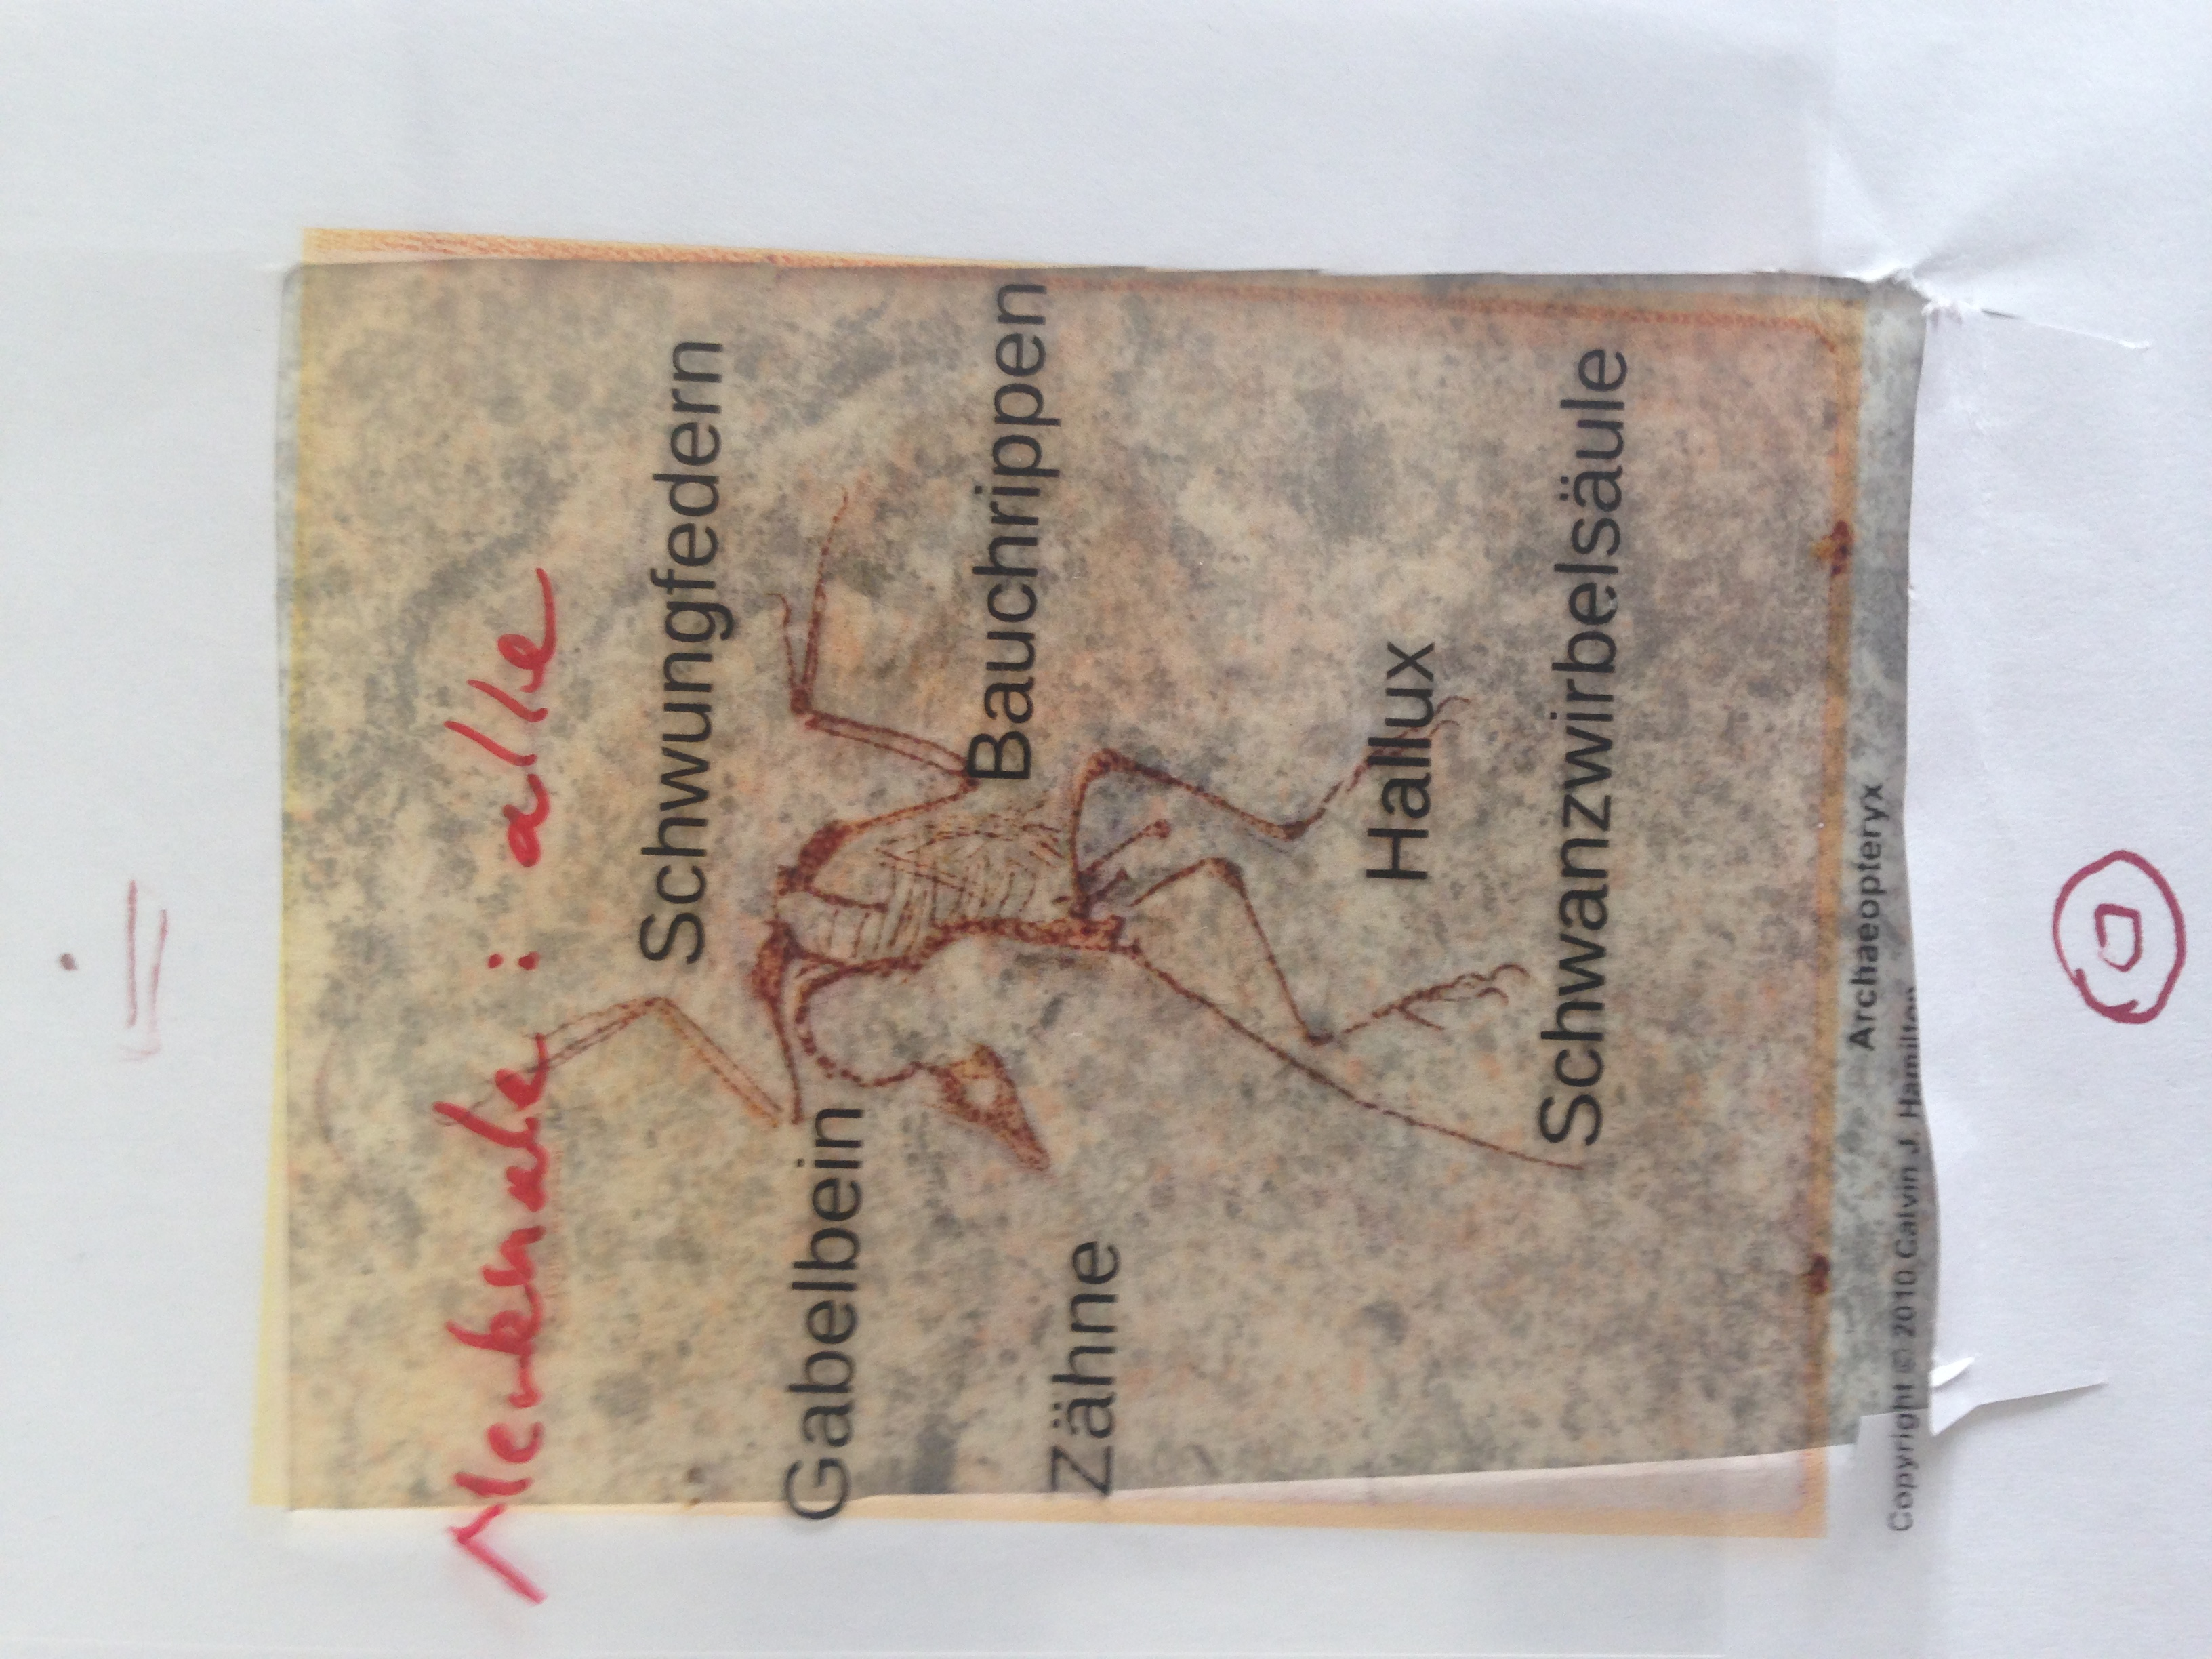
\includegraphics[angle=-90,scale=0.04]{proto}
	\caption{Mobile AR Anwendung}
	\label{fig:prototype}
\end{figure} 

Zur Umsetzung des Papierprototypen wurde beispielhaft der Archaeopteryx als Exponat gewählt. Mit der Anwendung sollen folgende Szenarien möglich sein, die in Abbildung \ref{pict:use_case} dargestellt sind.

\begin{figure}[H]
	\centering
	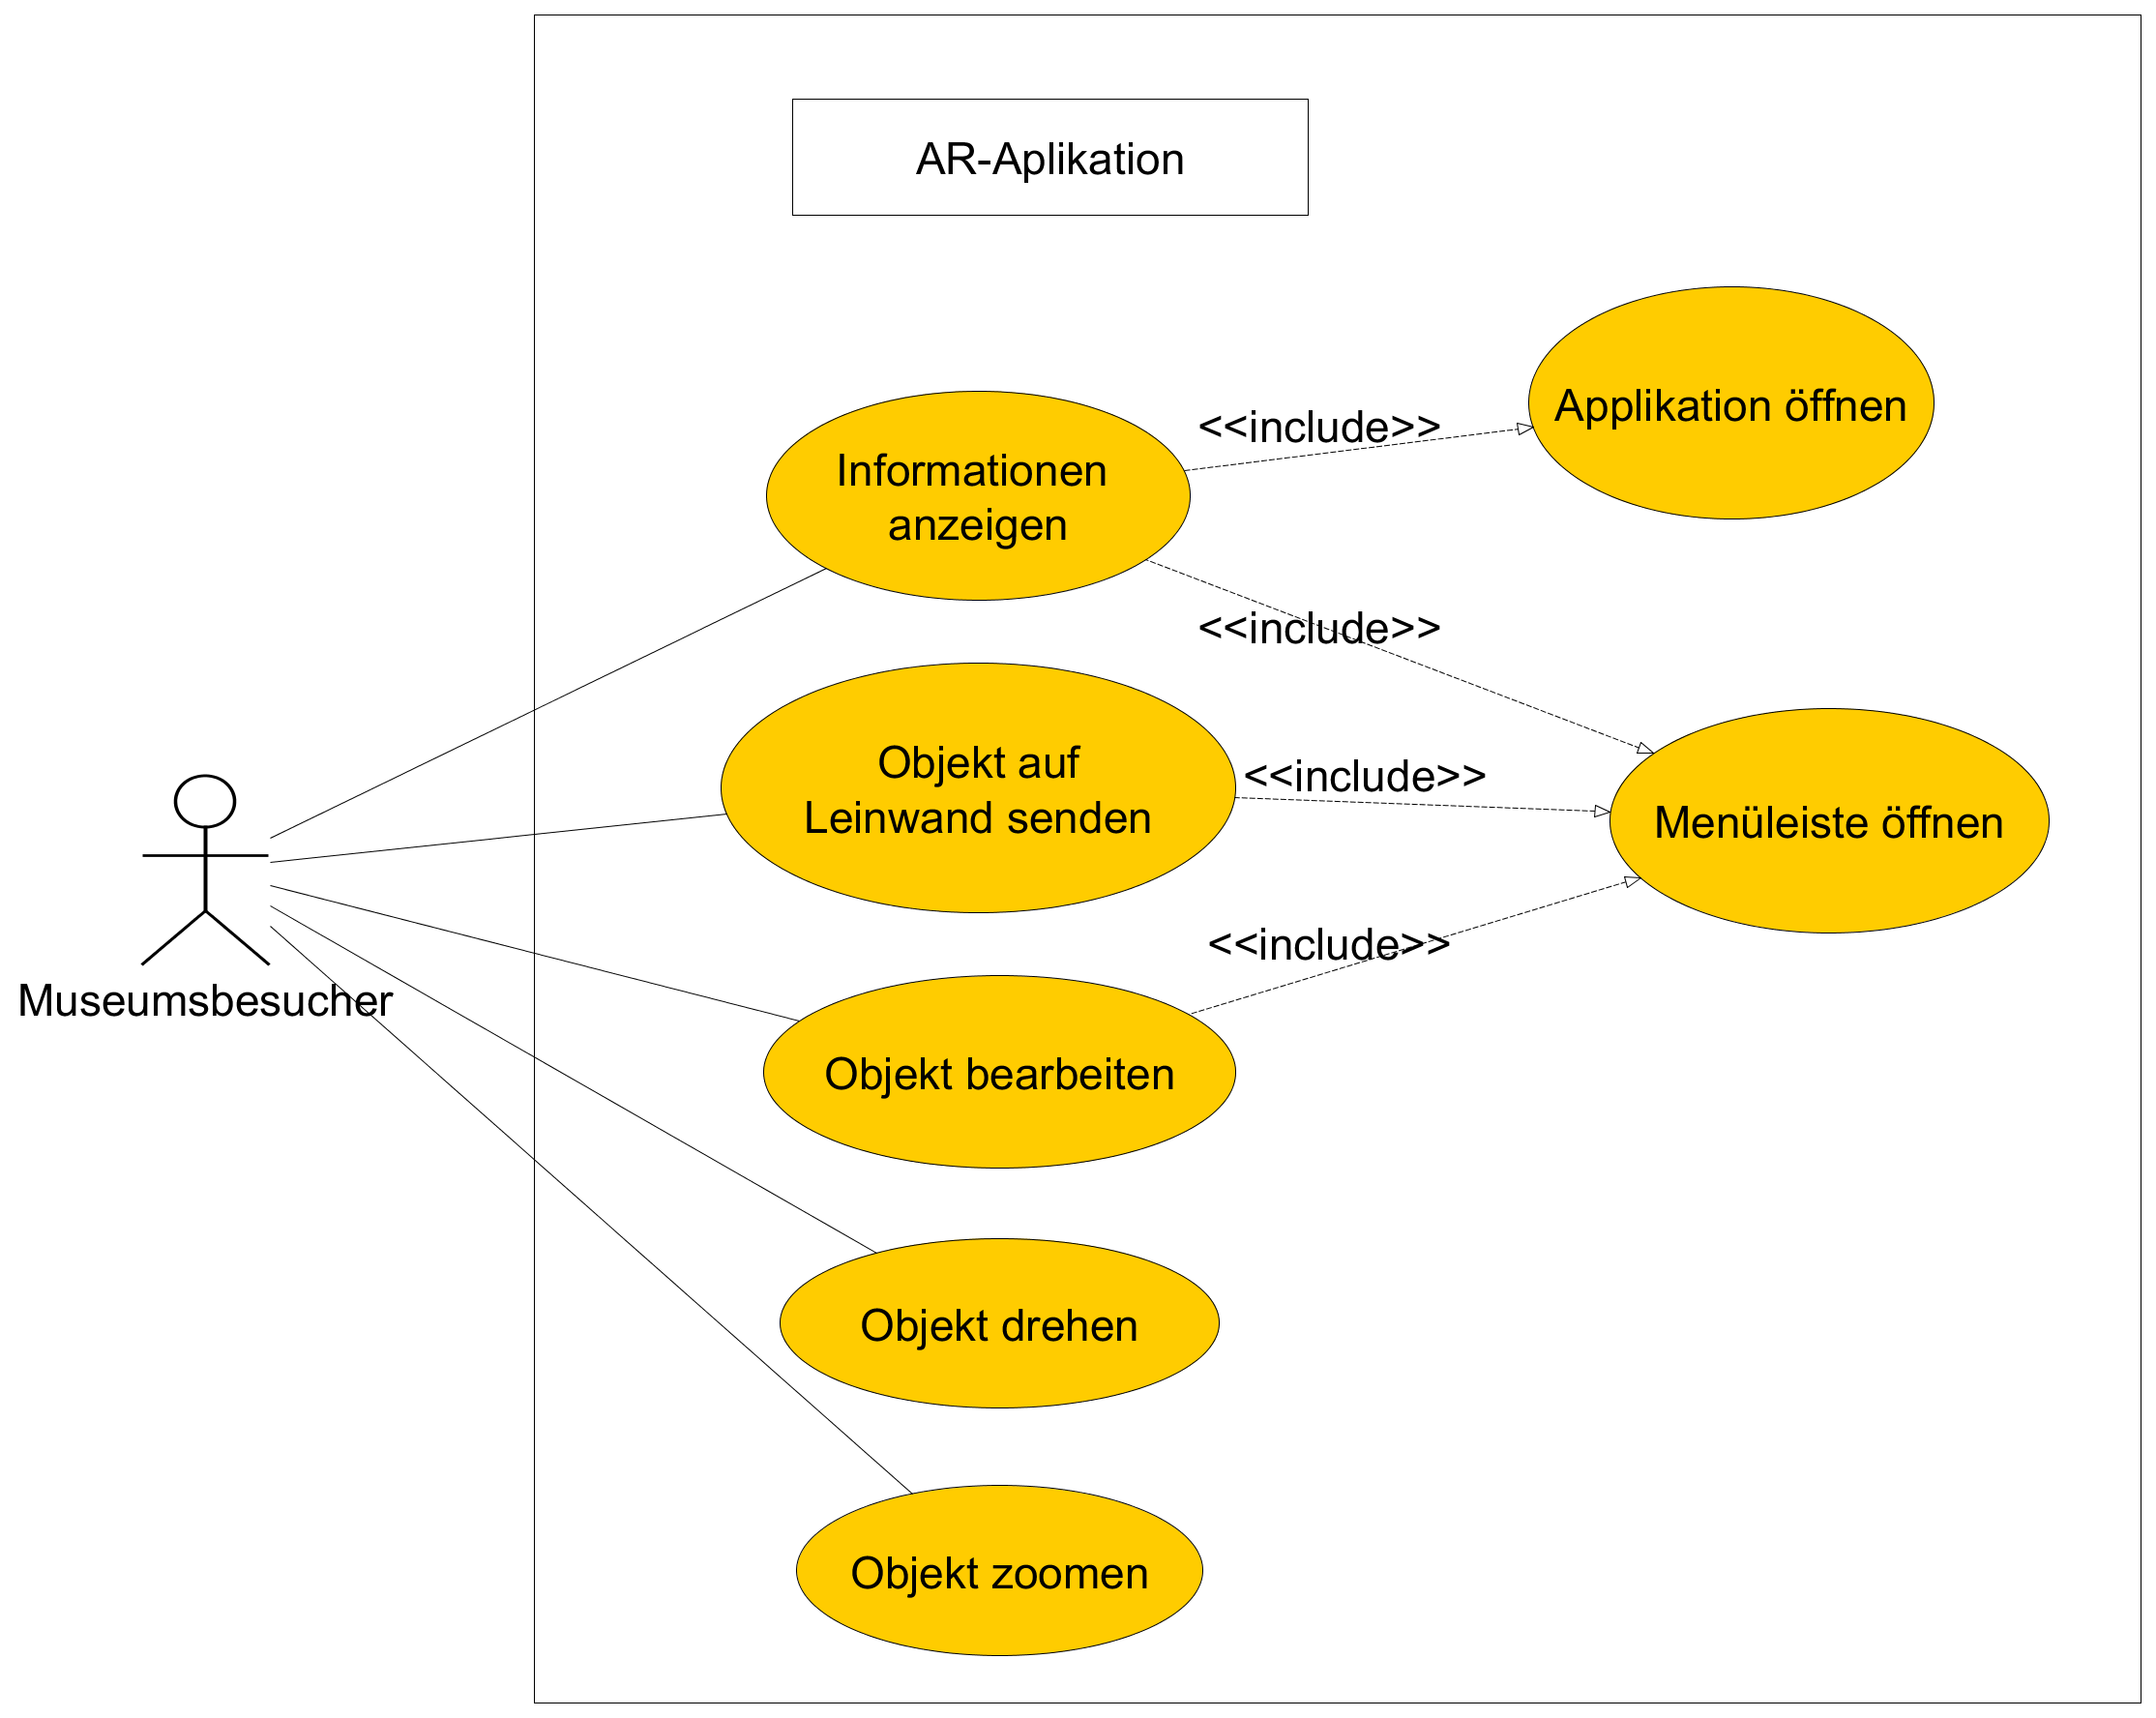
\includegraphics[scale=0.15]{use_c_museum}
	\caption{Use Case Diagramm: Mobile AR Anwendung}
	\label{pict:use_case}
\end{figure} 

Der Papierprototyp wurde für den Use Case Informationen anzeigen entwickelt, das den Use Case Exponat zoomen inkludiert. Die Gestaltung und Anzahl der Dialoge wurde bewusst minimal gehalten, um die Konzentration auf die Informationen lenken zu können. Die Interaktionen sollten aus den Informationen selbst erkennbar sein und durch bekannte Interaktionen umsetzbar sein. Als bekannte Interaktion ist das Zoomen mit Hilfe von zwei Fingern, die auseinander bzw. zusammen gezogen werden möglich. Ebenfalls als bekannt vorausgesetzt, ist das Zurücksetzten der Skalierung über das doppelte Tippen auf das Display. Nach dem Öffnen der Anwendung öffnet sich die Kamera. Der Nutzer soll im weiteren Schritt die Kamera auf das Exponat richten, sodass Informationen angezeigt werden können. Sobald das Exponat von der Kamera erfasst wurde, werden zu diesem Exponat allgemeine Informationen angezeigt, durch die gescrollt werden können durch das Wischen nach Oben bzw. Unten. Am Ende können über einen Button spezielle Informationen, wie die Merkmale des Archeopteryx angezeigt werden.
Für das Anzeigen von weiteren Informationen wird eine Slideshow umgesetzt. Die Benutzung der Slideshow erfolgt durch das Wischen nach Links und Rechts, wobei die Überschriften das Vorwissen des Nutzers anregen sollen, dass weitere Informationen durch das Wischen angezeigt werden können. Die Slideshow wurde nach den Grundsätzen der Dialoggestaltung nach der Erwartungskonformität gewählt. Die Slideshow dient zur Navigation, mit der sich mehrere Informationen zu einem Hintergrundbild, wie den Archeopteryx anzeigen lassen können.\\

\subsubsection{Prototyp Vorschlag II} \label{chapt:paperprotoII}
%TODO
%Einleitung zu Prototypen Varianten
In dieser zweiten Variante wurde eine mobile Anwendung entwickelt, die über die Kamera des mobilen AR-Gerätes mit dem Exponat interagiert. Mit Hilfe der Kamera kann das Exponat erfasst und die Ansicht um Informationen erweitert werden. Dabei werden zusätzlich auf dem Bildschirm  Informationen zu dem Exponat angezeigt. Nach dem Gesetz der Dialoggestaltung und dem Gesetz der Einfachheit zur Selbstbeschreibungsfähigkeit soll dem Nutzer durch aufsetzten der Brille erkennen, das er das Objekt zu dem er Informationen haben möchte Lediglich durch die Brille betrachten muss. Die Steuerbarkeit bezieht sich nur auf die Kopfhaltung und aus welcher Himmelsrichtung das Exponat betrachtet werden soll.. Abbildung \ref{fig:prototype_II} zeigt das Objekt durch die Brille erweitert mit spezifischen Informationen. Die  virtuellen Informationen zu dem Objekt sind um herum angelegt und können durch gescrollt oder geswitcht werden.  Die Gestaltung und Anzahl der angezeigten Informationen ist maximal minimalistisch Gehalten und soll dem Nutzer nicht auffallen. Das soll die Konzentration von der technischen Realisierung auf den entstehenden Komfort lenken. Eine Interaktion mit dem Exponat findet nicht direkt statt. Stattdessen soll der Text entsprechend der  vertikalen Kopfhaltung gescrollt werden.

\begin{figure}[H]
	\centering
	\includegraphics[angle=+90,scale=0.04]{proto_II}
	\caption{Prototyp II}
	\label{fig:prototype_II}
\end{figure} 

\begin{itemize}
	\item Die Anwendung wird gestartet wenn die AR-Brille aus der Halterung genommen bzw. angeschaltet wird.
	\subitem Das entsprechende Thema wurde vom Museum vorkonfiguriert und kann vom Benutzer nicht geändert werden. 
	\item Wenn der Nutzer im Umkreis eines Exponates ist, wird über dieses via AR zusätzliche Informationen angezeigt.
	\item Durch Heben oder Senken des Kopfes wird der eingeblendete Text gescrollt.
	\subitem Bei frei stehenden Exponaten können die angezeigten Informationen in 4 Blöcke aufgeteilt werden, wobei jeder einer Himmelsrichtung zugewiesen wird.
	\subitem Entsprechend der Ausrichtung des Users in Bezug auf die Himmelsrichtungen wird einer der 4 möglichen Informationsblöcke angezeigt.
	\item In der oberen linken Ecke soll eine MiniMap mit Positions-Kursor angezeigt werden
	\subitem die Karte soll halb transparent sein, um nicht zu aufdringlich zu wirken
	\item Die Anwendung wird beendet wenn dass Museumsgelände verlassen, das Device ausgeschaltet oder in die dafür vorgesehen Halterung zurückgesetzt.
	
\end{itemize}

\subsubsection{Prototyp Vorschlag III} \label{chapt:paperprotoIII}
%TODO
%Einleitung zu Prototypen Varianten
In dieser zweiten Variante wurde eine mobile Anwendung entwickelt, die über die Kamera des mobilen AR-Gerätes mit dem leeren Podesten interagiert. Mit Hilfe der Kamera kann das Podest erfasst und die Ansicht um ein Exponat sowie zugehörigen Informationen erweitert werden. Dabei werden zusätzlich auf dem Bildschirm ein entsprechendes Exponat(3D-Modell) und Informationen zu dem Exponat angezeigt. Nach dem Gesetz der Dialoggestaltung und dem Gesetz der Einfachheit zur Selbstbeschreibungsfähigkeit soll dem Nutzer durch aufsetzten der Brille erkennen, das er das Objekt und Information durch Betrachten der dafür vorgesehenen Podeste erreicht. Die Steuerbarkeit bezieht sich nur auf die Kopfhaltung und aus welcher Himmelsrichtung das Exponat betrachtet werden soll.
\\ Die Gestaltung und Anzahl der angezeigten Informationen ist maximal minimalistisch Gehalten und soll dem Nutzer nicht auffallen. Das soll die Konzentration von der technischen Realisierung auf den entstehenden Komfort lenken. Eine Interaktion mit dem Exponat findet nicht direkt statt. Stattdessen soll der Text entsprechend der  vertikalen Kopfhaltung gescrollt werden.
\\ Abbildung \ref{fig:prototype_III} zeigt einen Papierprototypen für die Umsetzung dieses Konzeptes.

\begin{figure}[H]
	\centering
	\includegraphics[angle=0,scale=0.04]{paper_protoIII}
	\caption{Ansicht Papierprototyp III}
	\label{fig:prototype_III}
\end{figure} 


\begin{itemize}
	\item Die Anwendung wird gestartet wenn die AR-Brille aus der Halterung genommen bzw. angeschaltet wird.
	\subitem Das entsprechende Thema wurde vom Museum vorkonfiguriert und kann vom Benutzer nicht geändert werden. 
	\item Wenn der Nutzer im Umkreis eines leeren Podestes steht und es anguckt, wird über dieses via AR ein Virtuelles Exponat erzeugt und mit den zusätzliche Informationen, angezeigt.\item Durch Heben oder Senken des Kopfes wird der eingeblendete Text gescrollt.
	\subitem Bei frei stehenden Exponaten können die angezeigten Informationen in 4 Blöcke aufgeteilt werden, wobei jeder einer Himmelsrichtung zugewiesen wird.
	\subitem Entsprechend der Ausrichtung des Users in Bezug auf die Himmelsrichtungen wird einer der 4 möglichen Informationsblöcke angezeigt.
	\item In der oberen linken Ecke soll eine MiniMap mit Positions-Kursor angezeigt werden
	\subitem die Karte soll halb transparent sein, um nicht zu aufdringlich zu wirken
	\item Die Anwendung wird beendet wenn dass Museumsgelände verlassen, das Device ausgeschaltet oder in die dafür vorgesehen Halterung zurückgesetzt.
	
\end{itemize}

Der Papierprototyp besteht aus einem Papiermodell einer Brille und ein-schiebbaren beschrifteten Papierstreifen um Inhalte wiederzugeben.
Die ein-schiebbaren Inhalte besitzen in der Mitte eine 30\% Breite vertikale Aussparung um die Sicht auf das Objekt nicht völlig zu verdecken.
Informationen werden durch ein Schiebesystem von oben nach unten eingeblendet. Die Ansichten sind auf einem fortlaufenden Papierstreifen notiert.
Die Podeste werden werden durch einfach Blätter Papier am Boden dargestellt, beschwert mit einem Simulationsobjekt wie z.B. ein Stift.





%TODO
%Adrians Prototyp Beschreibung plus Bild und deren Designentscheidung Bezug nehmen zur Vorlesung
%Zwei weitere Prototypen beschreiben und deren Designentscheidung Bezug nehmen zu Vorlesung; evtl zu jedem Prototyp ein Bild
%Nach den Grundsätzen der Dialoggestaltung
%Erwartungskonformität: Slideshow zur Navigation zu weiteren Informationen. Anzeige Punkte, die farblich hervorgehoben werden als Ankerpunkt. Wischen für weitere Informationen andere Ansicht. Scrollen Anzeige Scrollbar rechts. 

%Steuerbarkeit: 

%Selbstbeschreibungsfähig: App öffnet sich Kamera ist sofort an. Erklärt sich selbst, das auf Objekt gehalten werden muss, da Kamera an ist.

%Gesetz der Kontinuität:

%Gesetz der Verbundenheit:

%Gesetz der Einfachheit:

In der zweiten Variante der Papierprototypen wurde als zentrales Element ein tangible Interface verwendet. Zusätzlich zu dem TI, gibt es eine AR Brille mit einem Exponat und einem QR-Code. Die Brille ist in der Lage den QR-Code zu scannen um das Exponat virtuell auf der AR-Brille anzuzeigen. Das TI ist ein Kugelförmiges Gerät mit diversen verbauten Sensoren. Diese sind ein Gyrosensor, ein Beschleunigungssensor und ein Drucksensor.

\begin{figure}[H]
	\centering
	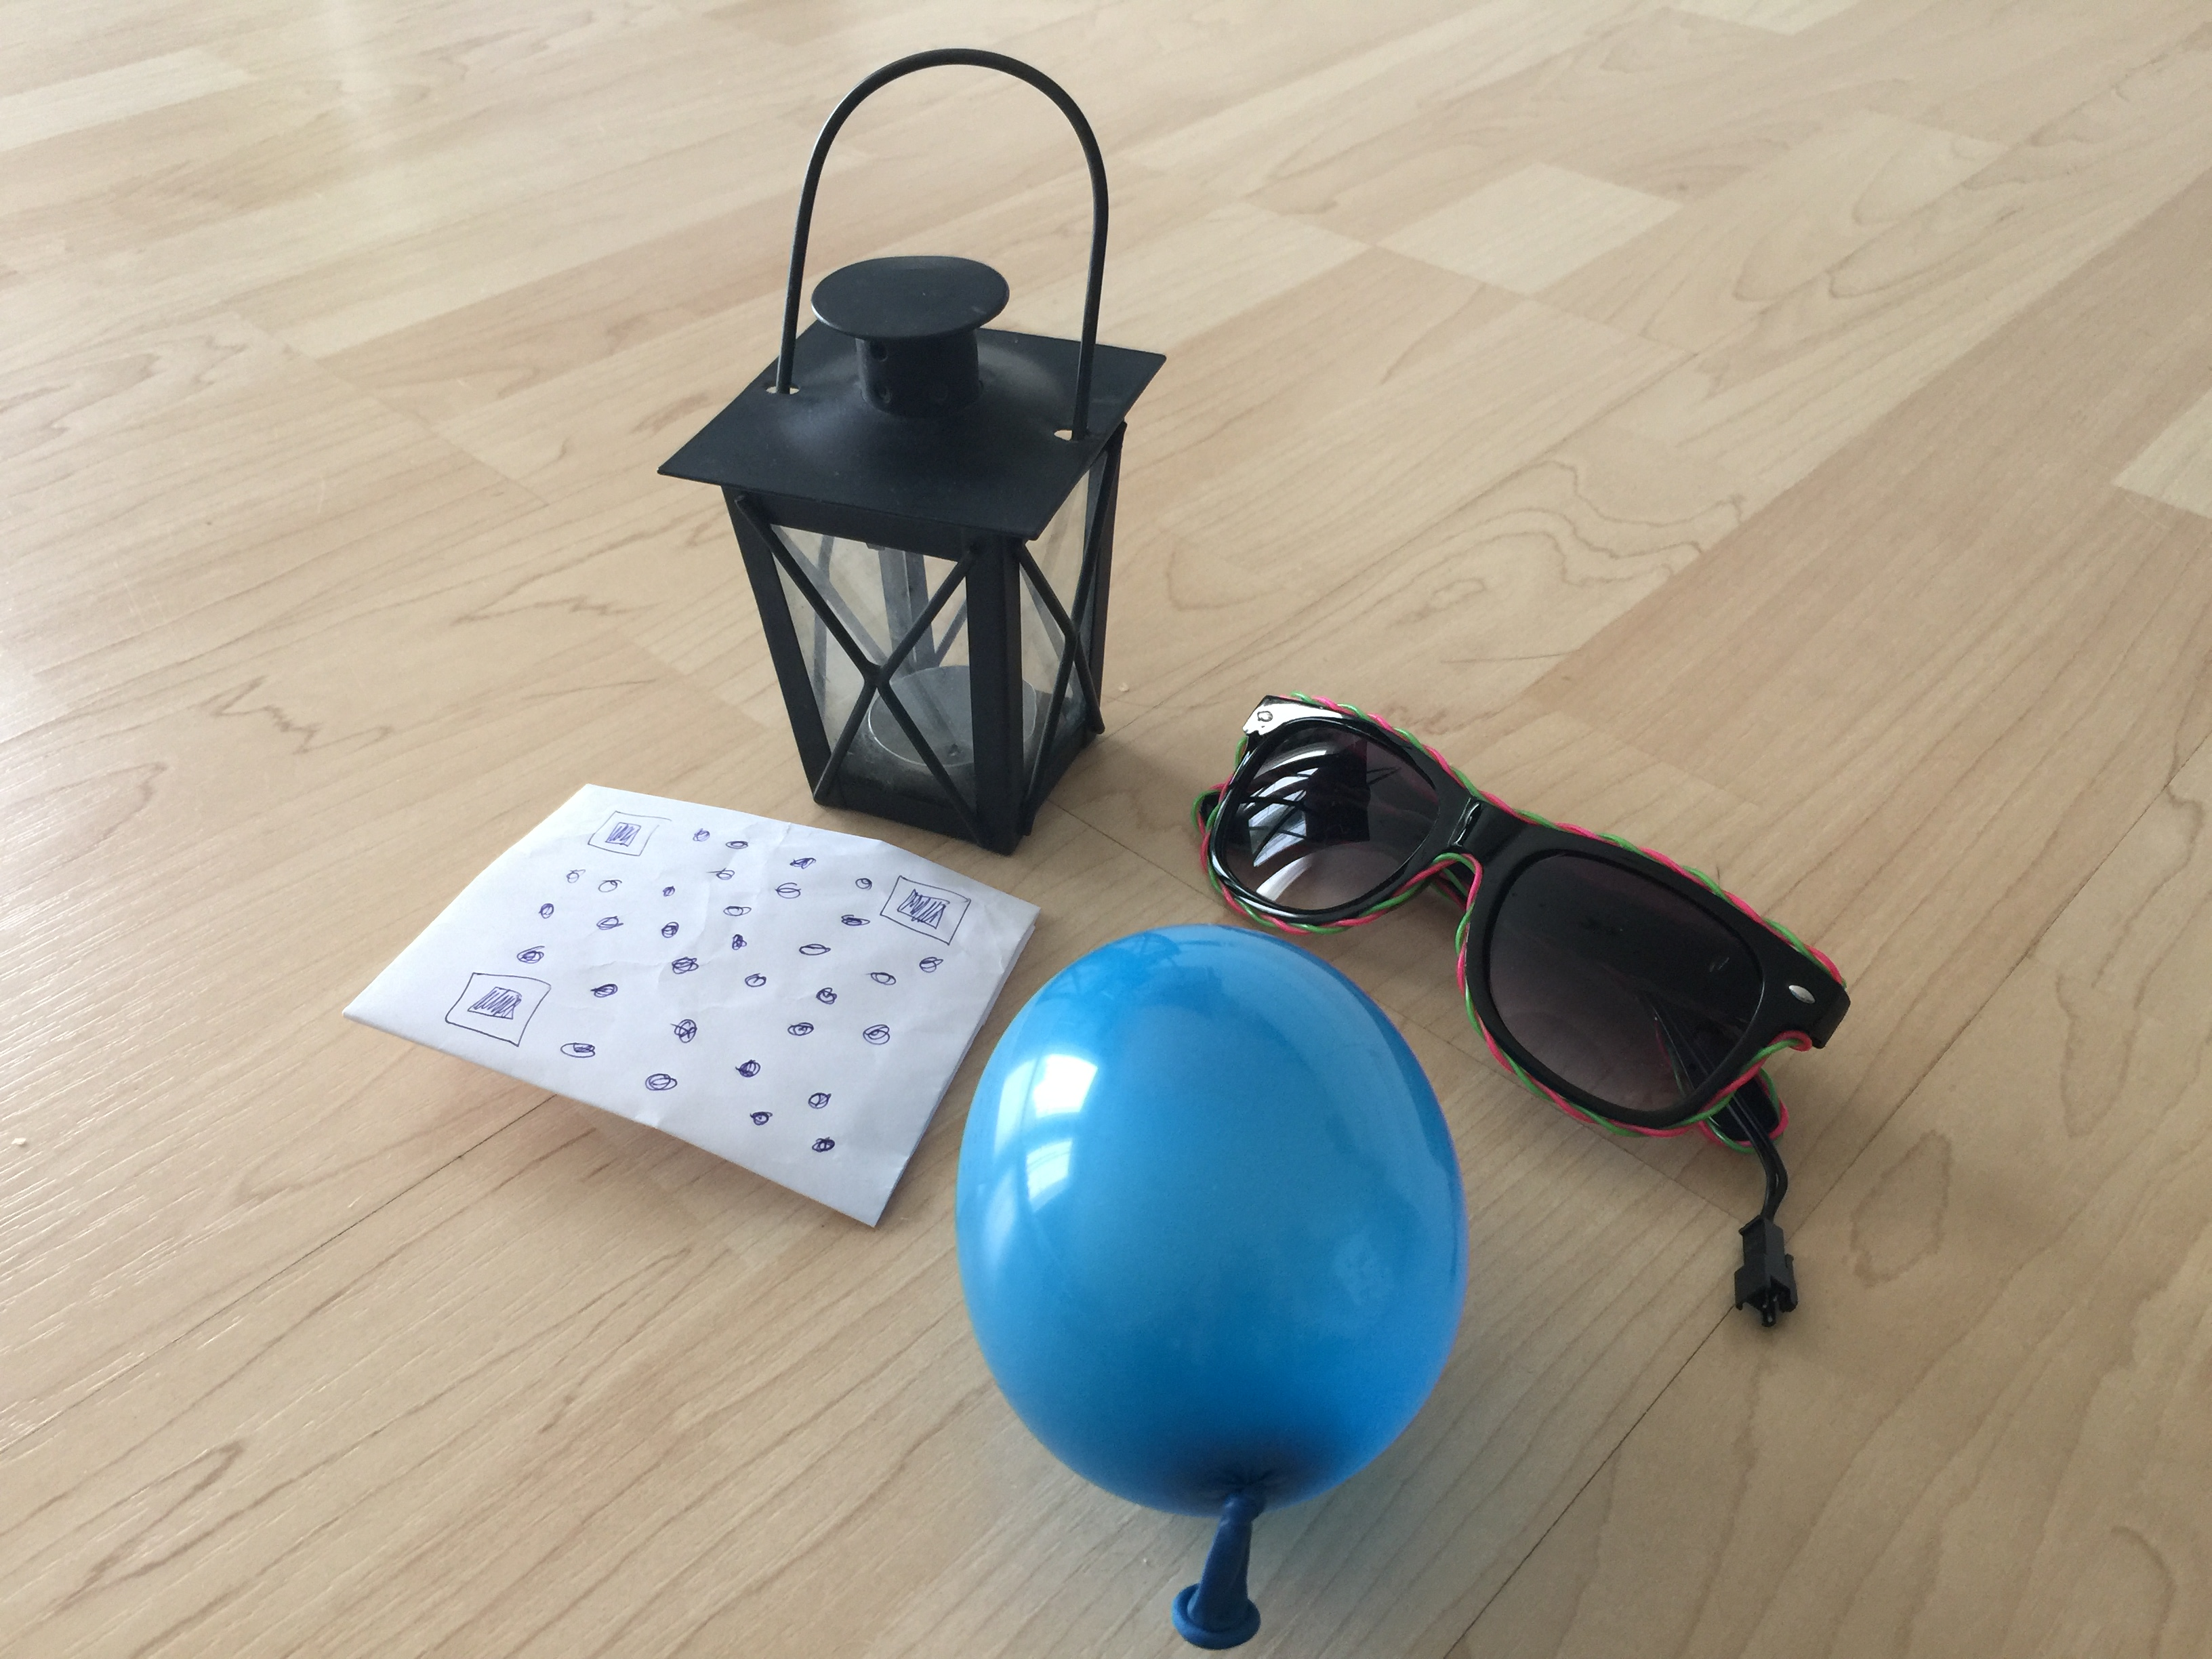
\includegraphics[angle=0,scale=0.04]{proto2}
	\caption{AR Anwendung mit TI}
	\label{fig:prototype2}
\end{figure}

Diser Usecase vernachlässigt hauptsächlich den informativen Teil wohin gegen die Userexperience im Vordergrund stehen soll.

\subsection{Heuristische Evaluation}
Die heuristische Evaluation wurde an der mobilen Anwendung zum Anzeigen von Informationen und der Anwendung zum Anzeigen von Exponaten als 3D-Objekt mit Hilfe eines Tangible Interface vollzogen. Um Usability Probleme zu entdecken, wurden die Heuristiken von Nielson verwendet. Damit lassen sich Eigenschaften des Systems herausfinden, die erfüllt sein müssen, damit die Interaktion für den Nutzer gebrauchstauglich sind.
Tabelle \ref{tab:heur_1} werden die Ergebnisse der heuristischen Analyse der mobilen Anwendung zusammengefasst.

\begin{table}
	\begin{tabular}{|c|c|c|c|}\hline
		\textbf{Dialog}		& \textbf{Erwartung}		&\textbf{Lösungsvorschlag}  & \textbf{Heuristik}\\
		\hline
		
							&  	\multirow{6}*{automatisches Scrollen} 	& Scrollbar einfügen &  \\
							
							& 											& zur Erkennung der	 & \\ 
							
		Allg. Information	& 										&Interaktionsmöglichkeit;&Sichtbarkeit\\
		
		anzeigen			&									&Umsetzen einer			&des Systemstatus\\
		
							& 											&automatischen 			&\\
							
							& 											& Wiedergabe			&\\
		\hline
		
							& \multirow{3}*{herangehen} 			& Info anzeigen 	&Übereinstimmung  \\
							
			Zoomen 			& 								& wie das Zoomen		&zwischen dem System\\
			
							& 								&funktioniert           & und der realen Welt\\
		\hline
		
				 			& \multirow{3}*{nicht erkannt} 	& Einfügen von			& Benutzerkontrolle, \\
				 			
		Wischen				& 											&Punkten zur Anzeige	& Hilfe und\\
		
							& 										&von Anzahl der Slides  & Dokumentation\\
		\hline		
					
	\end{tabular}\\
\caption{Ergebnisse heuristische Evaluation: mobile AR Anwendung}
\label{tab:heur_1}
\end{table}

Die Erwartung, das die allgemeinen Informationen automatisches gescrollt werden, beruht darauf, dass das System keine Rückmeldung über den Status zurückgegeben hat. Durch Einfügen einer Scrollbar wird dem Nutzer angezeigt, dass der Text nach unten hin bewegbar ist. Über die Größe des Rechtecks in der Scrollbar wird die aktuelle Position im Text angezeigt und ein Gefühl für die Länge des Textes gegeben.\\

Das System spricht nicht die Sprache des Nutzers beim Verwenden des Zoommechanismus. Durch die Verwendung der AR-Technologie hat der Nutzer das Gefühl, dass die Interaktion mit dem Objekt genauso funktioniert wie im reelen Leben. Dadurch wird erwartet, dass durch herangehen an das Exponat ein Zoomen möglich ist. Durch hinzufügen einer Informationshilfe wie das Zoomen anzuwenden ist, könnte der Nutzer die Interaktion lernen. Allerdings würde das der Heuristik von Nielson wiedersprechen, dass das System ohne Hilfe auskommen muss.\\

Das nicht erkennen der Funktion Wischen zum Anzeigen von weiteren Informationen lässt den Nutzer in eine Situation geraten aus die er nicht wieder zurück findet. Das wurde anhand der Heuristik Benutzerkontrolle festgestellt. Um die Funktion deutlich zu machen, am unteren Rand kleine Kreise dargestellt, die für jeweils eine Seite stehen. Die Kreise werden zusammen nebeneinander in gleichmäßigen Abstand positioniert, wobei der Kreis farbig dargestellt wird, der die Seite repräsentiert, die gerade angezeigt wird. Durch Wischen wird die nächste Seite angezeigt und der entsprechende Kreis farbig dargestellt. Eine direkte Auswahl der Seite, die angezeigt werden soll, kann durch das Tippen auf den Kreis vollzogen werden.\\

%TODO
%Adrians Ergebnisse der heuristischen Analyse  hier einfügen

\subsection{Fazit}
%fazit bezüglich der im digitalen Prototypen umzusetztenden Features
Nach der Durchführung der heuristischen Evaluation, entstand die Idee, die Funktionen  der mobilen AR Anwendung wie Zoomen, Scrollen, Drehen und Informationen anzeigen eines Objektes auf das Tangible Interface anzuwenden. Somit soll eine Anwendung zum Interagieren mit einem Exponat über ein Tangible Interface entstehen. Die Anwendung soll in zwei Modi verwendet werden können, die über einen Knopf gewechselt werden können. Im ersten Modus kann das Exponat angesehen, gedreht und vergrößert werden, im zweiten Modus können sich Informationen zu dem Exponat angezeigt werden lassen. Folgende Feature werden dafür umgesetzt:

\begin{itemize}
	\item Die Anwendung wird gestartet, wenn das Tangible Interface aus der Halterung am Terminal genommen wird.
	\item Beim Starten der Anwendung wird der Modus zum Interagieren geöffnet.
	\item Als Nutzer möchte ich das Exponat vergrößern, durch  Drücken des Tangible Interfaces. Dabei soll je nach Kraftaufwand eine entsprechende Skalierung stattfinden. 
	\item Als Nutzer möchte ich das Exponat drehen können, durch vertikales und horizontales Drehen des Tangible Interfaces.
	\item Als Nutzer möchte ich Informationen zu einem Exponat angezeigt bekommen, wenn ich den Informations-Knopf am Tangible Interface drücke.
	\item Als Nutzer möchte ich den Informationstext scrollen, durch vertikales Drehen des Tangible Interfaces.
	\item Als Nutzer möchte ich weitere Informationen anzeigen, durch horizontales Drehen des Tangible Interfaces.
	\item Als Nutzer möchte ich die angezeigten Informationen zu einem Exponat durch Drücken des Informations-Knopfes am Tangible Interface ausblenden.
	\item Die Anwendung wird durch Zurücklegen des Tangible Interfaces in das Terminal beendet.
	Wenn die Anwendung beendet wird, wird das Exponat ohne Zoom und Informationen angezeigt in einem voreingestellten Skalierungsmodus.
	
\end{itemize}

\section{Prototyping: high fidelity}
\subsection{Umsetzung des Papierprototypen}

Für die Umsetzung, nach eingehender Diskussion, sind im Team einige Neue Ideen entstanden. Zunächst wurde sich darauf geeinigt die grundlegenden Ideen der ersten beiden Prototypen zusammenzulegen.

\section{Zusammenfassung}


\newpage
\bibliographystyle{splncs03} 
\bibliography{bib}
\end{document}
